%%%%%%%%%%%%%%%%%%%%%%%%%%%%%%%%%%%%%%%%%%%%%%%%%%%%%%%%%%%%%%%%%%%%%%%
%%%
%%%         東京理科大学大学院 創域理工学研究科 機械航空宇宙工学専攻
%%%                   【非公式】修士論文要旨 テンプレート
%%%
%%%      <https://github.com/tsukahara-lab/TUS-ME_thesis_template>
%%%
%%%                                  v1.0.0 Yuki MATSUKAWA 15 Dec. 2021
%%%                                  v2.0.3 Yuki MATSUKAWA 27 Dec. 2023
%%%
%%%%%%%%%%%%%%%%%%%%%%%%%%%%%%%%%%%%%%%%%%%%%%%%%%%%%%%%%%%%%%%%%%%%%%%

%%% 文書クラスの設定 %%%
\documentclass[
    paper=a4paper,      % A4 用紙サイズ
    article,            % article 相当の文書クラス
    fleqn,              % 数式を左寄せ
    fontsize=12pt,      % 欧文サイズ 12 pt
    jafontsize=12pt,    % 和文サイズ 12 pt
    head_space=30mm,    % 天の余白
    foot_space=20mm,    % 地の余白
    gutter=18mm,        % のどの余白
    fore-edge=18mm      % 小口の余白
    ]{jlreq}            % jlreq クラスを使用

%%% abstract style %%%
% 修論要旨設定ファイル
\usepackage{settings_master}

% 行番号の表示
% 添削時には行番号を付けるとわかりやすい
% 提出時にはコメントアウトする
\linenumbers

\begin{document}

% 1 行あたり文字数の指定
\mojiparline{35}
% 1 ページあたり行数の指定
\linesparpage{30}

\begin{center}
% 修士論文題目
ここには修士論文のタイトルを入れます.\\ 一文字でも間違えたら受理されません.
% 修士論文題目
\end{center}

\vskip\baselineskip
\noindent
% 姓と名の間に「全角」スペース忘れずに
\begin{flushright}
    \begin{tabular}{r@{\hspace{3\zw}}r@{\hspace{0pt}\vspace{9pt}}}
        機械航空宇宙工学専攻 &
        % 自分の氏名を記入
        % \\ は消さない
        姓姓 名名 \\
        指導教員 &
        % 指導教員の氏名を記入
        姓姓 名名
    \end{tabular}
\end{flushright}

\vskip\baselineskip
%%% ここから書き始める %%%

% ダミーテキスト
\jalipsum[1-2]{wagahai}

図~\ref{fig:abst1} は虎,図~\ref{fig:abst2} も虎.

% ダミーテキスト
\jalipsum[1-4]{wagahai}

% 画像は 1, 2 枚程度にしておきましょう.
% 関連する図であれば (a), (b) にしてもいいでしょう.
\begin{figure}[b]
	\centering
	\begin{minipage}{0.35\columnwidth}
		\centering
		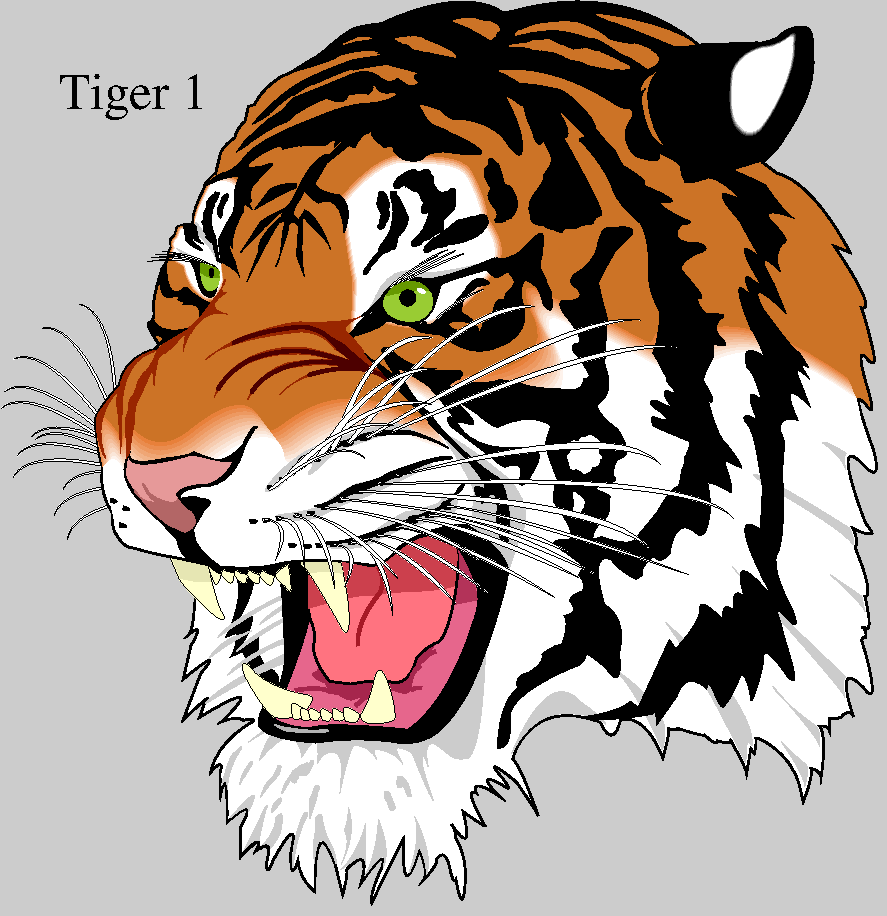
\includegraphics[width=\columnwidth]{tiger1.pdf}
		\caption{Tiger 1.}
		\label{fig:abst1}
	\end{minipage}
	\hspace{10mm}
	\begin{minipage}{0.35\columnwidth}
		\centering
		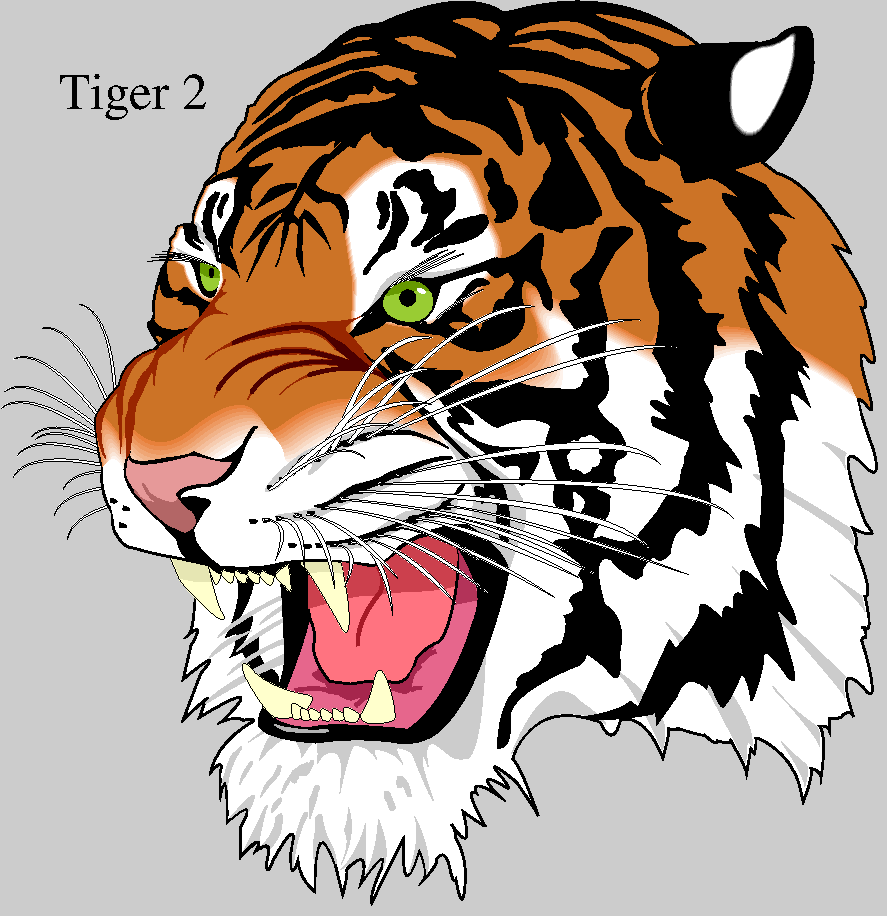
\includegraphics[width=\columnwidth]{tiger2.pdf}
		\caption{Tiger 2.}
		\label{fig:abst2}
	\end{minipage}
\end{figure}

%%% ここまで %%%

\end{document}
